\chapter{Método de trabajo}
\label{chap:metodo}

\drop{E}{}sta sección está centrada en detallar y justificar la metodología usada durante la elaboración del proyecto, de tal forma que se exponga al lector cómo ha sido llevado a cabo el desarrollo a nivel organizativo. Conjuntamente, se especifican los medios hardware y software que han sido utilizados a lo largo de todo el \acs{TFG}.

\section{Metodología}
\label{sec:metodologia}

Para la elección de la metodología de trabajo se debe escoger una que se ajuste a las condiciones del proyecto, es decir, que satisfaga la dinámica de trabajo que se desea seguir. Por lo cual es primordial que la metodología elegida divida el \textbf{desarrollo en hitos} que son potencialmente entregables y que no contienen errores. Igualmente, se debe tener en consideración el contexto donde se desarrolla el sistema. En este proyecto, al tiempo que se realiza el desarrollo del sistema es plausible que aparezcan complicaciones, por lo que es preciso que la metodología sea flexible, en otras palabras, que sea posible corregir las tareas con respecto a los inconvenientes que aparecerán durante el progreso del proyecto, conservando como línea de referencia los objetivos precisados (Referenciar Capitulo de objetivos).

En consecuencia, se excluyen las metodologías de desarrollo tradicionales, basadas en una planificación inicial que permanece intacta de principio a fin. Se decide escoger una \textbf{metodología de desarrollo ágil} cuyo principal objetivo es desarrollar proyectos de forma \textbf{iterativa e incremental}, en la que puedan definirse objetivos en cada iteración. La preferencia sobre una metodología ágil posibilita la entrega, en un periodo de tiempo reducido, de un proyecto funcional y que el usuario pueda evaluar. Entre las metodologías de desarrollo ágil existe un amplio abanico donde elegir: Programación Extrema, Desarrollo Adaptativo de Software, Scrum, etcétera. De ellas, \textbf{Programación Extrema} es la que mejor se ajusta a las exigencias del proyecto.

\subsection{Manifiesto ágil}
\label{sec:manifiestoagil}

Para comprender mejor la filosofía tras las metodologías ágiles, seguidamente se cita el \textbf{Manifiesto Ágil} \footnote{\url{http://www.agilemanifesto.org/iso/es/}} y sus cuatro valores:

«Estamos descubriendo formas mejores de desarrollar software tanto por nuestra propia experiencia como ayudando a terceros. A través de este trabajo hemos aprendido a valorar:

\begin{itemize}
\item \textbf{Individuos e interacciones} sobre \textbf{procesos y herramientas}.
\item \textbf{Software funcionando} sobre \textbf{documentación extensiva}.
\item \textbf{Colaboración con el cliente} sobre \textbf{negociación contractual}.
\item \textbf{Respuesta ante el cambio} sobre \textbf{seguir un plan}.
\end{itemize}

Esto es, aunque valoramos los elementos de la derecha, valoramos más los de la izquierda». De estos cuatro valores, se desarrollaron doce principios para el Manifiesto Ágil \footnote{\url{http://agilemanifesto.org/iso/es/principles.html}}, que son:

\begin{itemize}
\item La mayor prioridad es \textbf{satisfacer al cliente} mediante la entrega temprana y continua de software con valor.
\item \textbf{Aceptar} que los \textbf{requisitos cambien}, incluso en etapas tardías del desarrollo. Los procesos Ágiles aprovechan el cambio para proporcionar ventaja competitiva al cliente.
\item Se \textbf{entrega} software funcional \textbf{frecuentemente}, entre dos semanas y dos meses, con preferencia al periodo de tiempo más corto posible.
\item Los \textbf{responsables} de negocio, en este caso David Vallejo como director del proyecto, y los \textbf{desarrolladores trabajan juntos} de forma cotidiana durante todo el proyecto.
\item Los proyectos se desarrollan en torno a \textbf{individuos motivados}. Hay que darles el entorno y el apoyo que necesitan, y confiarles la ejecución del trabajo.
\item El método más eficiente y efectivo de \textbf{comunicar información} al equipo de desarrollo y entre sus miembros es la conversación \textbf{cara a cara}. 
\item El \textbf{software funcionando} es la \textbf{medida principal de progreso}.
\item Los procesos Ágiles promueven el \textbf{desarrollo sostenible}. Los promotores, desarrolladores y usuarios debemos ser capaces de mantener un ritmo constante de forma indefinida.
\item La \textbf{atención continua} a la excelencia técnica y al buen diseño \textbf{mejora la Agilidad}.
\item La \textbf{simplicidad}, o el arte de maximizar la cantidad de trabajo no realizado, \textbf{es esencial}.
\item Las mejores arquitecturas, requisitos y diseños emergen de \textbf{equipos auto-organizados}.
\item A intervalos regulares \textbf{el equipo reflexiona sobre cómo ser más efectivo} para a continuación ajustar y perfeccionar su comportamiento en consecuencia. 
\end{itemize}

\subsection{Programación Extrema}
\label{sec:progextrema}

La \textbf{Programación Extrema} (\acs{XP}) «requiere que se complete algún tipo de producto potencialmente liberable al final de cada iteración. Estas iteraciones están diseñadas para ser cortas y de duración fija. Este enfoque en entregar código funcional cada poco tiempo significa que el desarrollador no tiene tiempo para teorías. No persiguen dibujar el modelo UML perfecto en una herramienta CASE, escribir el documento de requisitos perfecto o escribir código que se adapte a todos los cambios futuros imaginables. En vez de eso, el desarrollador se enfoca en que las cosas se hagan. Se acepta que puede equivocarse por el camino, pero también es consciente de que la mejor manera de encontrar dichos errores es dejar de pensar en el software a un nivel teórico de análisis y diseño y sumergirse en él, ensuciarse las manos y comenzar a construir el producto» \cite{scrum}.

Por consiguiente, se puede definir \acs{XP} como una metodología de desarrollo ágil que persigue el objetivo de aumentar la productividad a la hora de desarrollar programas. Este modelo de programación se basa en una serie de metodologías de desarrollo de software en las que se da prioridad a los trabajos que dan un resultado directo y que reducen la burocracia que hay alrededor de la programación.

El \textbf{ciclo de vida ideal de \acs{XP}} según \cite{scrum2} consiste en seis fases:

\begin{itemize}
\item \textbf{Exploración}: los clientes, en este caso David Vallejo como director del proyecto, plantean a grandes rasgos las historias de usuario que son de interés para la primera entrega del producto. Al mismo tiempo el desarrollador se familiariza con las herramientas, tecnologías y prácticas que se utilizarán en el proyecto.
\item \textbf{Planificación de la entrega}: el cliente establece la prioridad de cada historia de usuario, y correspondientemente, los programadores realizan una estimación del esfuerzo necesario de cada una de ellas. Se toman acuerdos sobre el contenido de la primera entrega y se determina un cronograma en conjunto con el cliente.
\item \textbf{Iteraciones}: incluye varias iteraciones sobre el sistema antes de ser entregado. El plan de entrega está compuesto por iteraciones de no más de tres semanas. En la primera iteración se puede intentar establecer una arquitectura del sistema que pueda ser utilizada durante el resto del proyecto. Al final de la última iteración el sistema estará listo para entrar en producción.
\item \textbf{Producción}: requiere de pruebas adicionales y revisiones de rendimiento antes de que el sistema sea trasladado al entorno del cliente. Al mismo tiempo, se deben tomar decisiones sobre la inclusión de nuevas características a la versión actual, debido a cambios durante esta fase.
\item \textbf{Mantenimiento}: el proyecto XP debe mantener el sistema en funcionamiento al mismo tiempo que desarrolla nuevas iteraciones. Para realizar esto se requiere de tareas de soporte para el cliente.
\item \textbf{Muerte del proyecto}: cuando el cliente no tiene más historias para ser incluidas en el sistema. Se genera la documentación final del sistema y no se realizan más cambios en la arquitectura.
\end{itemize}

La utilización de \acs{XP} en el proyecto tiene un conjunto de ventajas asociadas:
\begin{itemize}
\item El proceso de \textbf{integración es continuo}, por lo que el esfuerzo final para la integración es nulo.
\item Se consiguen productos con mayor \textbf{rapidez}.
\item El desarrollo iterativo hace que los proyectos sean \textbf{adaptables} y abiertos a la incorporación de cambios.
\end{itemize}

\section{Herramientas}
\label{sec:herramientastfg}

\subsection{Hardware}
\label{sec:hardware}

Este \acs{TFG} tiene un elevado componente hardware, siendo los siguiente medios (ver Figura~\ref{fig:hardware}) los destinados a su elaboración:

\begin{itemize}
\item \textbf{Computador Packard Bell EN-TS44HR}.
\item \textbf{Quadcopter 3DR IRIS+} (véase Sección \ref{sec:3driris}): 3DR IRIS+ hace uso de:
	\begin{itemize}
	\item \textbf{Piloto automático Pixhawk} (véase Sección \ref{sec:pixhawk}).
	\item \textbf{Tarot T-2D Gimbal} \footnote{\url{https://store.3dr.com/products/tarot-t-2d-brushless-gimbal-kit}}: asegura tener imágenes estables y claras desde el vehículo.
	\item \textbf{Kit de telemetría Flug51 FL1515} a 433 MHz: proporciona una manera fácil de configurar una conexión entre el Pixhawk y una estación terrestre.
	\item \textbf{Sistema radiocontrol FlySky FS-TH9X} \footnote{\url{http://www.flysky-cn.com/products_detail/&productId=42.html}}: sistema extremadamente versátil que permite controlar el 3DR IRIS+ y puede ser usado por principiantes y expertos.
	\end{itemize}
\item Cámara \textbf{GoPro HERO 3+ Silver Edition} \footnote{\url{https://es.gopro.com/support/hero3plus-silver-support}}: permite la visualización de imágenes, así como la grabación de las mismas.
\item \textbf{Kit \acs{FPV}} \footnote{\url{http://www.robotshop.com/media/files/pdf/user-manual-vidkit0007.pdf}}: incluye todo lo necesario para empezar a emitir en directo imágenes a distancia y en primera persona de la GoPro acoplada al 3DR IRIS+. Para su utilización es necesario:
	\begin{itemize}
	\item \textbf{LogiLink USB 2.0} \footnote{\url{http://www.logilink.eu/showproduct/VG0001A.htm?seticlanguage=en}}: su función es digitalizar la señal de vídeo. \\
	\end{itemize}
\end{itemize}

\begin{figure}[!h]
\begin{center}
\subfigure[Maleta para transportar el 3DR IRIS+]{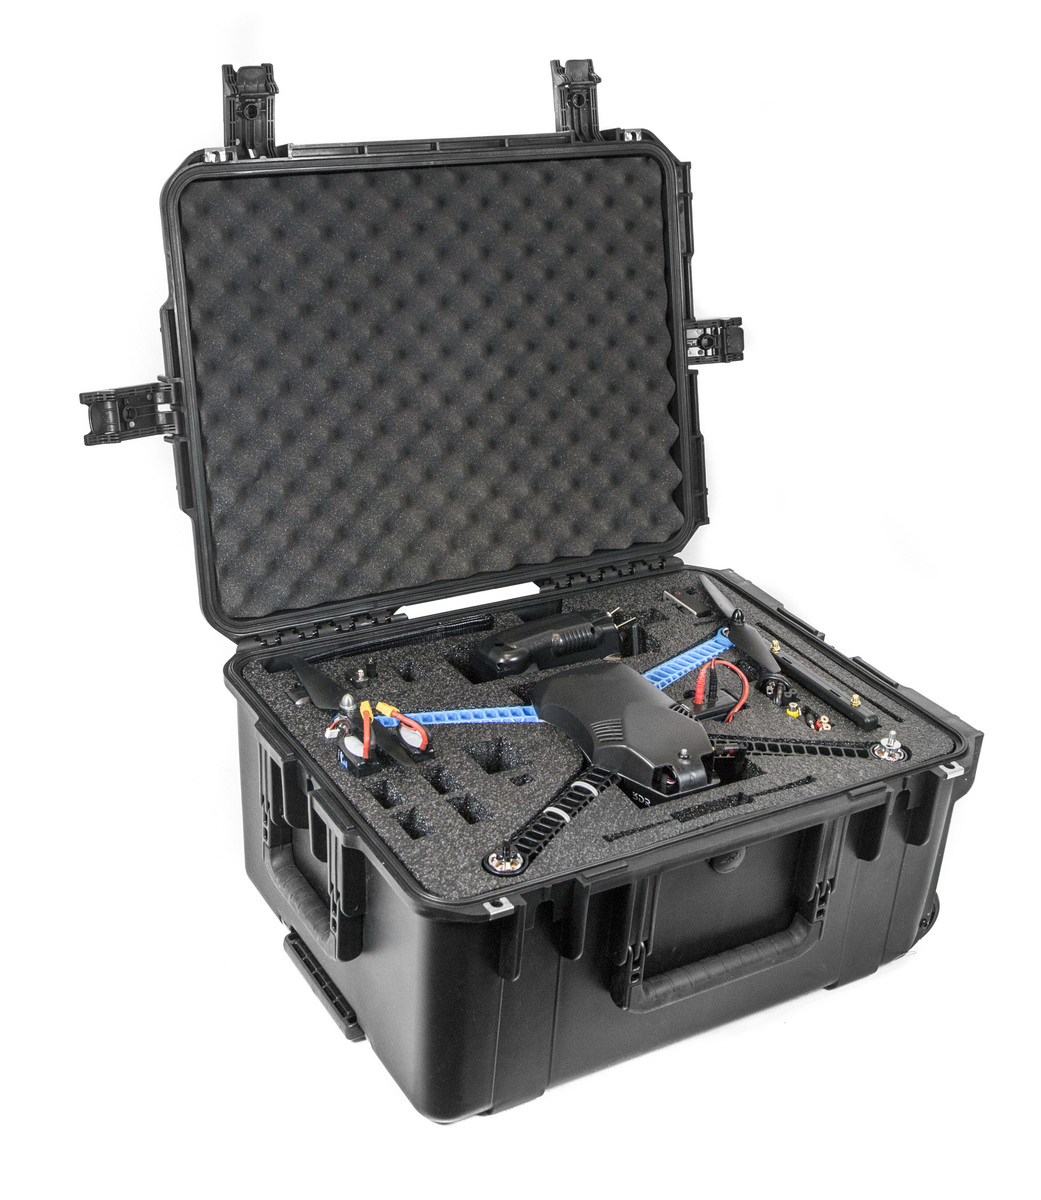
\includegraphics[width=0.4\textwidth]{/maleta.jpg}}
\subfigure[Tarot T-2D Gimbal con GoPro HERO 3+]{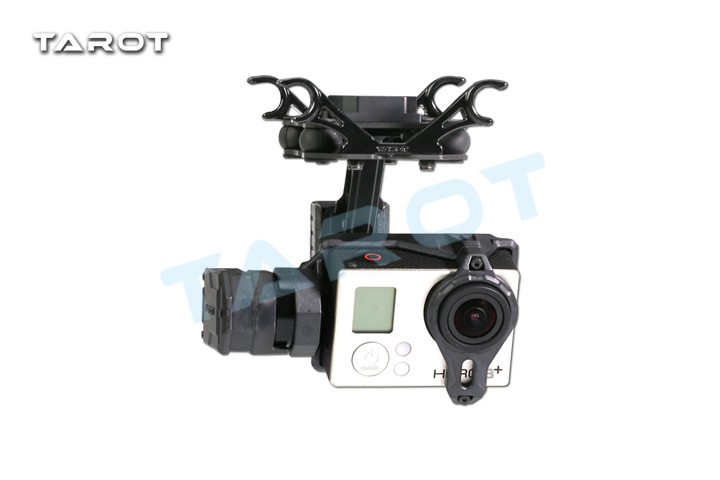
\includegraphics[width=0.5\textwidth]{/gimbal.jpg}}
\subfigure[Kit \acs{FPV}]{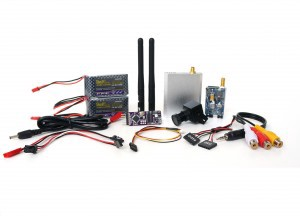
\includegraphics[width=0.5\textwidth]{/kitfpv.jpg}}
\subfigure[Kit de telemetría FL1515]{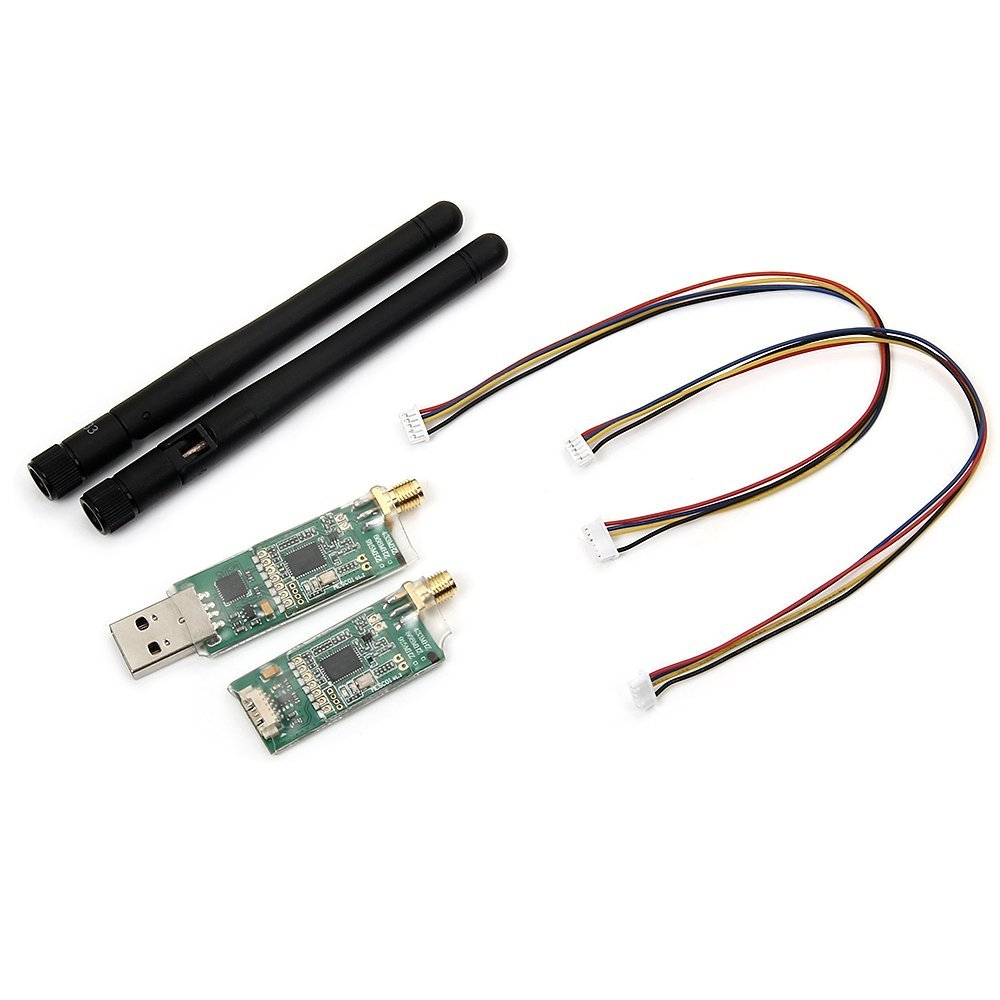
\includegraphics[width=0.3\textwidth]{/telemetria.jpg}}
\subfigure[3DR IRIS+, FS-TH9X y batería LiPo]{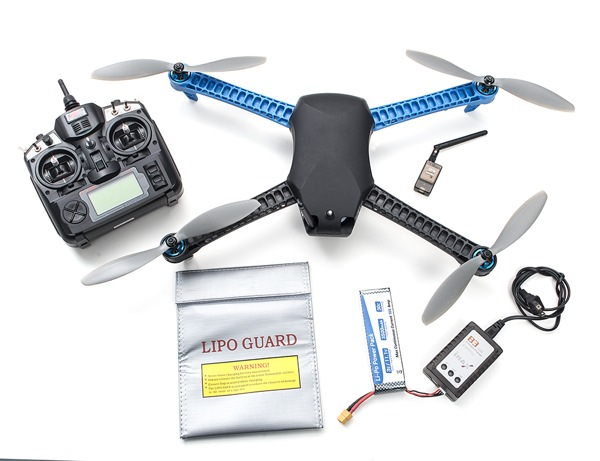
\includegraphics[width=0.5\textwidth]{/3drcompleto.jpg}}
\subfigure[LogiLink USB 2.0]{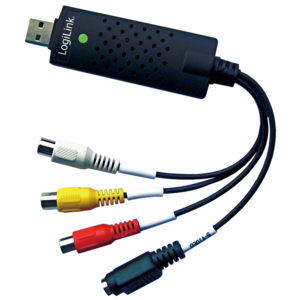
\includegraphics[width=0.3\textwidth]{/logilink.png}}
\caption[Ejemplo de medios hardware empleados durante el \acs{TFG}]{Ejemplo de medios hardware empleados durante el \acs{TFG}}
\label{fig:hardware}
\end{center}
\end{figure}

\clearpage

\subsection{Software}
\label{sec:software}

Para el desarrollo del proyecto se ha hecho uso de los siguientes medios software:

\subsubsection{Sistema operativo \acs{GNU}/Linux Ubuntu 14.04 \acs{LTS}}
\label{sec:ubuntu}

\textbf{Ubuntu} \footnote{http://www.ubuntu.com} fue concebido en 2004 por Mark Shuttleworth, un exitoso emprendedor sudafricano, y su compañía Canonical. Es una distribución \acs{GNU}/Linux que ofrece un sistema operativo que está disponible de forma libre y cuenta con apoyo de la comunidad de usuarios y con soporte profesional.

La comunidad Ubuntu se basa en las ideas consagradas en el \textbf{Manifiesto Ubuntu} \footnote{\url{http://www.ubuntu.com/about/about-ubuntu/our-philosophy}}: \textbf{i)} el software deberá estar siempre disponible \textbf{sin costo} alguno, \textbf{ii)} dicho software podrá ser utilizado en la lengua materna del usuario y a pesar de cualquier discapacidad y \textbf{iii)} los usuarios siempre tendrán la \textbf{libertad de adaptar} y modificar el software de acuerdo a sus necesidades particulares. Esta libertad es la que hace a Ubuntu radicalmente diferente del software propietario tradicional.

Ubuntu es apropiado tanto para ordenadores de escritorio como para servidores. Incluye más de 1.000 paquetes entre los cuales se incluyen el kernel de Linux y Gnome. También se incluyen las aplicaciones que se esperan en cualquier ordenador de escritorio, como procesador de texto, hoja de cálculo y navegador para Internet. Por lo tanto, su uso es apto en el ámbito doméstico, profesional o educativo. 

\subsubsection{\LaTeX}
\label{sec:latex}

Para la confección del presente documento se ha utilizado \textbf{\LaTeX} \footnote{\url{https://www.latex-project.org/}}. \LaTeX es un sistema de preparación de documentos para la composición tipográfica de alta calidad. Con frecuencia se utiliza para documentos técnicos o científicos, pero se puede utilizar para casi cualquier forma de publicación.

El término \LaTeX hace referencia solo al \textbf{lenguaje} en que estos documentos son escritos, pero no al editor para escribirlos. Para generar un documento en \LaTeX, un archivo .tex debe ser creado empleando un editor de textos y posteriormente será compilado para producir, en este caso, un \textbf{archivo PDF}. Cualquier editor puede ser utilizado para crear un documento \LaTeX, pero existen también algunos editores específicos para trabajar con \LaTeX.

La idea de \LaTeX es que el autor se \textbf{concentre en el contenido de lo que escribe}, en lugar de la presentación visual. Al preparar un documento \LaTeX, el autor especifica la estructura lógica usando conceptos familiares como: capítulo, sección, tabla, figura, etc; dejando al sistema \LaTeX preocuparse de la presentación visual de esas estructuras.

\subsubsection{\acs{GNU} Emacs}
\label{sec:emacs}

Para la creación de documentos en \LaTeX y para implementar el código fuente, \textbf{\acs{GNU} Emacs} ha sido el editor de texto empleado. \acs{GNU} Emacs es un editor de textos avanzado que es auto-documentado, extensible y personalizable. Su núcleo es un intérprete de Emacs Lisp, un dialecto del lenguaje de programación Lisp con extensiones para la edición de texto. 

Emacs se considera un editor de textos avanzado porque puede hacer mucho más que la simple inserción y eliminación de texto. Puede controlar subprocesos, programas de sangría automática, mostrar varios archivos a la vez, y mucho más. 

\textbf{Auto-documentado} significa que en cualquier momento se pueden utilizar comandos especiales, conocidos como comandos de ayuda, para averiguar cuáles son sus opciones, o para averiguar lo que hace cualquier orden. \textbf{Personalizable} significa que se puede alterar fácilmente el comportamiento de los comandos de Emacs. Y \textbf{extensible} significa que puede ir más allá de la personalización sencilla y crear nuevos comandos.

\subsubsection{Git}
\label{sec:git}

Para el control de versiones se ha optado por el software \textbf{Git} \footnote{\url{https://git-scm.com/}}. El proyecto se ha alojado en un repositorio online de \textbf{Github} \footnote{\url{https://www.github.com}}, que es un servicio gestionado por el sistema de control de versiones Git.

El control de versiones es un sistema que \textbf{registra los cambios} de un archivo, o un conjunto de archivos, a largo del tiempo, para poder recordar versiones específicas más adelante. Permite revertir los archivos de nuevo a un estado anterior, comparar los cambios durante el transcurso del proyecto o ver quién modificó algo que podría ser la causa de un problema.

Git es un \textbf{sistema distribuido de control de código fuente} diseñado por Linus Torvalds, pensando en la eficiencia y la confiabilidad del mantenimiento de versiones de aplicaciones cuando estas tienen un gran número de archivos de código fuente. Ayuda a los programadores a ser más eficientes en el trabajo, ya que ha universalizado las herramientas de control de versiones que no estaban tan popularizadas y tan al alcance de los desarrolladores.

\subsubsection{APM Planner 2.0}
\label{sec:planner}

\textbf{APM Planner} es una aplicación de estación de tierra con todas las funciones necesarias para el proyecto de piloto automático de código abierto Ardupilot.

APM Planner es una \textbf{estación de control de tierra} para aviones, helicópteros y vehículos. Es compatible con Windows, Linux y Mac OSX. Puede ser usado como una utilidad de configuración o como un complemento de control dinámico para el vehículo autónomo. \\

Entre las tareas que APM Planner puede realizar están las siguientes:
\begin{itemize}
\item \textbf{Cargar el firmware} en el piloto automático.
\item \textbf{Instalar, configurar y ajustar} el vehículo para mejorar el rendimiento.
\item \textbf{Introducción de «waypoints»} mediante point-and-click, usando Google Maps,Bing u Open Street Maps.
\item \textbf{Selección de comandos} de misión mediante desplegables.
\item \textbf{Descarga y análisis} de los archivos de \textbf{log} de misión.
\item Con el hardware de telemetría adecuado puede:
	\begin{itemize}
	\item \textbf{Supervisar el estado} del vehículo mientras está funcionando.
	\item \textbf{Grabar registros} de telemetría.
	\item Ver y \textbf{analizar estos registros} de telemetría.
	\item Hacer funcionar su vehículo en \textbf{\acs{FPV}}.
	\end{itemize}
\end{itemize}

\subsubsection{Software in the Loop}
\label{sec:sitl}

La simulación permite realizar pruebas de seguridad de código y ajustes experimentales, además de servir para practicar el uso de la estación de tierra desde el escritorio. \textbf{\acs{SITL}} consigue simular helicópteros, aviones o vehículos terrestres sin la necesidad de ningún hardware. Su ejecución es posible en Windows, Linux y Mac OSX.

\acs{SITL} es una reproducción del código del piloto automático utilizando un compilador C++, resultando esto en un ejecutable que posibilita \textbf{probar el comportamiento del código sin hardware}. El simulador \acs{SITL} permite ejecutar ArduPilot en su computador directamente, sin ningún hardware especial. Esto es porque aprovecha el hecho de que ArduPilot es un piloto automático portátil que puede funcionar en una variedad muy amplia de plataformas, siendo el ordenador otra plataforma en la que ArduPilot puede ser ejecutada.

Una gran ventaja de ArduPilot en SITL es que le da acceso a toda la gama de herramientas de desarrollo disponibles, como depuradores interactivos, analizadores estáticos y herramientas para el análisis dinámico. Esto hace que el desarrollo y prueba de nuevas funciones en ArduPilot sea mucho más sencillo.

\subsection{Lenguajes}
\label{sec:lenguajes}

\subsubsection{Python 2.7.6}
\label{sec:python}

El lenguaje principal para el desarrollo de este proyecto es \textbf{Python} \footnote{\url{https://www.python.org/}}, ya que se dispone de un \acs{SDK} en este lenguaje, como es DroneKit-Python (véase Sección \ref{sec:dronekit}), que facilitará la implementación considerablemente.

Python es un lenguaje de propósito general, de alto nivel, interpretado y que admite la aplicación de diferentes paradigmas de programación, como por ejemplo, la programación procedural, la programación imperativa o la \textbf{programación orientada a objetos}. Es ideal para prototipado rápido, pero también permite el desarrollo de grandes aplicaciones. Su filosofía de diseño enfatiza la legibilidad del código y su sintaxis permite al programador expresar los conceptos en menos líneas que en otros lenguajes. Se trata de un lenguaje potente, flexible y con una sintaxis clara y concisa.

Python puede ser utilizado en diversas plataformas y sistemas operativos, entre los que podemos destacar los más populares, cómo Windows, Linux y Mac OSX. Además, dispone de un excelente conjunto de \textbf{librerías para extender su funcionalidad}, incluyendo librerías científicas que permiten realizar numerosas tareas de tratamiento de datos, visualización, cálculo numérico y simbólico y otras aplicaciones específicas.

% Local Variables:
% coding: utf-8
% mode: latex
% mode: flyspell
% ispell-local-dictionary: "castellano8"
% End:
